\documentclass[11pt,letter]{article}
\usepackage[utf8]{inputenc}
\usepackage{amsmath}
\usepackage{amsfonts}
\usepackage{amssymb}
\usepackage{enumitem}
\setlist[enumerate]{itemsep=0mm}
\setlength\parindent{0pt}
\usepackage{graphicx}
\usepackage{verbatim}


\author{Haosu Tang}
\title{Project C}
\usepackage[margin=1in]{geometry}

\begin{document}

\maketitle

\section{1.Beta}
I chose BA (Boeing company) to do this analysis. Data range: 2008-01-01 to 2009-12-31, during which the financial crisis happened and the market was highly volatile.

(a). Time series plots of the 3-month rolling beta, S\&P 500 and scatter plot of beta vs S\&P500.
\begin{center}
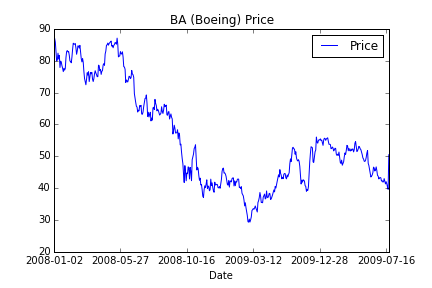
\includegraphics[width=4in,keepaspectratio]{1aBA}
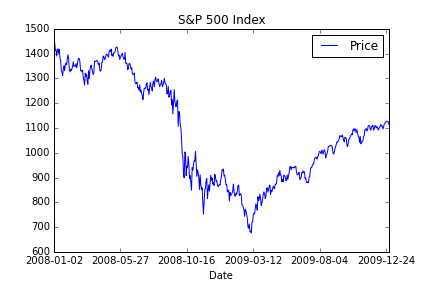
\includegraphics[width=4in,keepaspectratio]{1aSP}
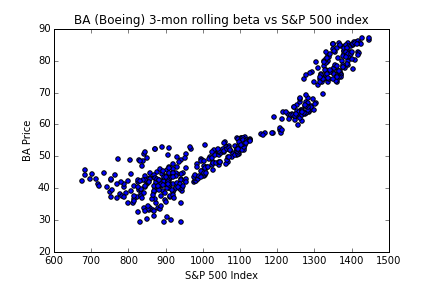
\includegraphics[width=4in,keepaspectratio]{1aBASPscatter}
\end{center}

(b). A scatter plot of 1-day stock returns vs. the SPTR 1-day return and the linear regression fitting line.
\begin{center}
\includegraphics[width=4in,keepaspectratio]{1aBARetSPTRscatter}
\end{center}
Equation for linear regression:
\begin{itemize}
\item (With intercept): $ \hat{y} = -0.00041234 + 0.92471118 \hat{x}$
\item (Intercept = 0): $ \hat{y} = 0.92509641 \hat{x}$
\end{itemize}

(c). A scatter plot of 1-day stock returns vs. the VIX 1-day return and the linear regression fitting line.
\begin{center}
\includegraphics[width=4in,keepaspectratio]{1aBARetVIXscatter}
\end{center}
\begin{itemize}
\item (With intercept): $ \hat{y} = -0.00084599 -0.23941314 \hat{x}$
\item (Intercept = 0): $ \hat{y} = -0.23939968 \hat{x}$
\end{itemize}


\section{2.Performance attribution}
(a) Using data from strategy "Contra01" from OLAP database for 2005-2009, analyze the performance. I plotted the "Weighted Return Tc" and "1 month Volatility" for this period. To note, "1 month Volatility" and "3 month Volatility" have exactly the same 


%
%
%
%(a). Plot and label a bar graph with the time series of daily portfolio returns and one with the time series of daily market returns.
%
%I used Access to get equity universe data from obelix.mit.edu and query it to form a table consisting of:
%\begin{enumerate}
%\item date d, an integer number starting from 7543 to 10570, representing trading dates between 1/1/1990 and 12/31/2001,
%\item stock id, if the flag is 1,
%\item log return r.
%\end{enumerate}
%
%And using Matlab, for each day, 
%\begin{enumerate}
%\item transform the log return to real return,
%\item calculate mean return and each stock's absolute return,
%\item assgin normalized weight to each stock,
%\item calculate the portfolio return through dot product $pi_t= w_{t-1}^TR_t$.
%\end{enumerate}
%(The code is attached at the end of this write-up.)
%
%The time series plot for the return of the mean reversion portfolio:
%
%\begin{center}
%\includegraphics[width=4in,keepaspectratio]{Mean_rev}
%\end{center}
%
%And comparing to the time series plot for the return of the market:
%
%\begin{center}
%\includegraphics[width=4in,keepaspectratio]{Market}
%\end{center}
%
%(b). The mean annualized return, volatility, and Sharpe ratio of the strategy and of the market average. The annualized return I calculated using compounded return and then annualize: $\sqrt[n]{\Pi(1+r_i)}-1$. Volatility is simply overall daily standard deviation multiplied by $\sqrt{252}$ (252 trading days). And Sharpe ratio is calculated by dividing the annualized return by volatility, assuming risk free rate 0.
%\begin{verbatim}
%strat_Annu_r = 22.164171668343567
%
%strat_Annu_vol = 0.213763539224245
%
%strat_Annu_SR = 1.036854636145064e+02
%
%market_Annu_r = 0.169325792411088
%
%market_Annu_vol = 0.092115857155619
%
%market_Annu_SR = 1.838182888805254
%\end{verbatim}
%
%(c). Consistency and stationarity: Time series consistency and stationarity is defined as preserving a constant mean throughout time and having a time-independent well defined autocovariance. Judging from the the two time series plots, there is not serial correlation and clustering effect, and for both cases the means and covariances are more or less constant. However, the market variances do seem a bit inflated between 2000-3000 (about 1997-2001), suggesting a more volatile market. Therefore, the consistency and stationarity can be assumed valid in this case for ease of analysis, but the increase in variance one should bear in mind.
%
%\begin{center}
%\includegraphics[width=4in,keepaspectratio]{Mean_rev_refline}
%\end{center}
%
%(d). I define unusual outlier dates as those larger than $\bar{R} \pm 4S$, where $S$ is the standard deviation. Under the assumption of returns being normally distributed, a 4 standard deviation away is less than 0.001\% likely. The results are:
%\begin{verbatim}
%[7713, 7863, 8032, 8457, 8458, 9174, 9484, 9817, 9840, 10092, 10448, 10486]
%\end{verbatim}
%
%These correspond to these dates:
%09/04/1990, 04/09/1991, 12/06/1991, 08/12/1993, 08/13/1993, 06/13/1996, 09/04/1997, 12/30/1998, 02/03/1999, 02/02/2000, 07/02/2001, 08/24/2001.\\
%
%And I defined the outlier stocks as the assigned weight of more than 10\%, which means for the previous day, this stock behaves abnormally (either extremely high return or extremely low return) against the market average. These stocks and the corresponding weights are:
%\begin{verbatim}
%   63511: 0.113350040847314
%   30761: 0.147599964114200
%   55336: 0.119772746634528
%   48389: 0.100088821163926
%   61524: 0.108428751055292
%   66545: 0.107852786103411
%   34841: 0.135585573246371
%\end{verbatim}
%
%These outlier dates and stocks will have an effect on overall stock returns as it scales the return of the total portfolio and gets magnified throughout the time series.
%
%(e) The correlation between the strategy and the market:
%\begin{verbatim}
%corr(strategy, market) = 0.069865960126031
%\end{verbatim}
%To test whether or not the strategy is market-neutral, I ran a counter-example: I revert all the market returns to their negative and keep the strategy unchanged. In this case, the market is downward trending in the time frame, however, the strategy is able to yield the same return after all.
%\begin{verbatim}
%strat_Annu_r2 = 22.164171668343528
%
%market_Annu_r2 = -0.152124918872277
%
%corr(strategy, market2) = -0.069865960126031
%\end{verbatim}
%As can be seen from this circumstance, the market return is now negative, but the strategy return remains positive unchanged. Essentially, the "Mean reversion strategy" after all is related to the trend in the market and bet it to be reverting and is thus unchanged in this case. And the correlation is now negative. This suggests the strategy is also market neutral.\\
%
%(f) The correlation between long and short positions. It is calculated by recording long positions and short positions individually and finding the correlation:
%\begin{verbatim}
%corr(long, short) = -0.261439839425657
%\end{verbatim}
%
%(g) This simulation is purely imaginary and cannot be realistic due to a number of reasons. Some are:
%\begin{enumerate}
%\item \textbf{Trading cost.} To rebalance a daily portfolio of 690 stocks induces extremely high trading costs. The high return will definitely not sustain under this condition.
%
%\item \textbf{Slippage.} In this simulation I used daily return, while in real time it would not be the case. It is very hard to bet on the price one wants and slippage may occur due to multiple reasons (timing, unfilled orders etc).
%
%\end{enumerate}
%
%Counting various factors, my guess of the annualized return should be much lower than the market return - this strategy cannot beat the market. It is hard to find a actual number. The idea is the daily return of the simulation is approximately 1.2\%, but then the trading cost of 690 stocks would account for approximately $690*2*0.01\%$ assuming 0.01 transaction cost. This yields high negative return! The data issues need to be considered related to the strategy is incompleteness of data, possible wrongly recorded data, null/NaN data, and requirement for finer data.
%
%\section{A family of strategies.}
%
%$k$ from 1 to 10:\\
%
%\begin{tabular}{l | l l l}
%k & Return & Volatility & Sharpe Ratio\\
%\hline
%1 & 22.16 & 0.2138 & 103.69 \\
%2 & 0.3593 & 0.1493 & 2.407\\
%3 & 0.2019 & 0.1441 & 1.401\\
%4 & 0.1382 & 0.1332 & 1.037\\
%5 & 0.04871 & 0.1354 & 0.3596\\
%6 & 0.1642 & 0.1363 & 1.2051\\
%7 & 0.01336 & 0.1280 & 0.1044\\
%8 & 0.09610 & 0.1293 & 0.7430\\
%9 & 0.01090 & 0.1266 & 0.08611\\
%10 & 0.00009533 & 0.1292 & 0.0007377\\
%\end{tabular}
%\newline
%\newline
%There is a significant decreasing trend in return, which suggests mean reversion feature dies out with time.\\
%
%Uploaded to Obelix. Access sql query is extremely painful - took more than 6 hours to map t to d.\\
%
%Check results:\\
%1. Row numbers of ID 919122398:\\
%\includegraphics{check1}\\
%2. Check 10 rows:\\
%\includegraphics{check2}
%
%\includegraphics[width=4in,keepaspectratio]{check1}

\end{document}